\chapter{Reconnaissance automatique des émotions : corpus et méthodes}
\label{chapitre3}
«Si vous voulez être libre de vos émotions il faut avoir la connaissance réelle, immédiate de vos émotions.»  (Arnaud Desjardins, 1925-2011)


\section{Le domaine de la reconnaissance automatique des émotions}
Le domaine de la reconnaissance automatique des émotions, ou Speech Emotion Recognition (SER) se concentre sur les tâches de reconnaissance des différents états émotionnels d'un ou de plusieurs locuteurs. Ce domaine est en pleine expansion grâce notamment à l'utilisation de nouveaux systèmes neuronaux empruntés à d'autres domaines du Machine Learning.
Afin de mettre en place des expérimentations sur ces tâches de reconnaissance et de caractérisation des émotions, il est important de mettre en place des données pertinentes sur lesquelles s'appuyer, des méthodes pour représenter efficacement ces données ainsi que de mettre en place des systèmes d'évaluation robustes permettant de comparer les différentes expérimentations.

\section{Les corpus existants}
Aujourd'hui, les tâches de reconnaissance d'émotion sont principalement traitées en tant que tâches supervisées : le système apprend à reconnaître des étiquettes émotionnelles associées à des segments de parole à partir de corpus de parole annotés en émotions.

\subsection{Les différents types de corpus}
\subsubsection{Corpus actés}
Comme nous l'avons vu dans le premier chapitre de cette thèse, la caractérisation de l'état émotionnel d'une personne peut être assez délicate, puisqu'elle est en grande partie subjective. De plus, il est communément admis que l'expression des états émotionnels sont ponctuels et rares dans la parole. Pour pallier ce problème, on peut construire des corpus dit \textit{actés}. Il s'agit de corpus où l'état émotionnel n'est pas naturel.

On fait alors appel à des acteurs, qui vont simuler des états émotionnels dictés par le responsable de l'élaboration du corpus. Par exemple, les acteurs devront dire le mot \textit{hippopotame} de façon joyeuse, triste puis avec dégoût. Cette pratique est très utilisée pour avoir différents états émotionnels d'un même locuteur, le tout rapidement. Elle est à privilégier quand on recherche l'exhaustivité des états émotionnels chez un sujet. Ces corpus sont aujourd'hui toujours majoritaires. On peut notamment citer les corpus Emo-Db~\cite{Burkhardt2005} et DES~\cite{Engberg1997}. L'inconvénient principal d'un tel protocole est que les émotions obtenues sont prototypiques dans leur manifestation, les rendant difficile à comparer à des émotions dites \textit{naturelles}. De plus, l'utilisation d'acteurs peut se révéler coûteuse.

\subsubsection{Corpus induits}
Un autre type de corpus utilisé dans la reconnaissance d'émotion est le corpus induit. On utilise différentes méthodes pour induire les états émotionnels que l'on souhaite étudier.

Une des méthodes pour construire ce genre de corpus est d'utiliser un \textit{magicien d'Oz} abrégé WoZ (\textit{Wizard of Oz}). Cette méthode consiste à simuler un dialogue homme-machine, où la machine est en fait complètement commandée par un opérateur humain, qui va simuler une réponse de machine. Ainsi l'humain pense avoir affaire à un serveur vocal ou un robot, alors que c'est l'opérateur qui est responsable des réponses engendrées par le système.

On peut également parler de la recherche de stress par laquelle on peut placer les sujets dans des situations stressantes comme des montagnes russes~\cite{Hansen1997} ou une prise de parole en public~\cite{Giraud2013}. Quant à la tristesse, on peut utiliser des extraits de films par exemple~\cite{Schuller2010cinemo}. Ces émotions sont plus proches des émotions réelles, elles sont donc moins manifestes.

Les corpus actés et induits ont pour avantage d'être créés dans des environnements contrôlés et permettent de rendre les données facilement accessibles. Ces données sont, la plupart du temps, produites à des fins d'analyse. Il est donc facile de recueillir le consentement des participants avant la mise en place de l'expérience, de contrôler la qualité des enregistrements et la cohérence des données en contraignant les participants sur un sujet ou à exprimer un type d'état émotionnel défini. Néanmoins ils ne représentent pas la vie réelle, sont souvent de petite taille et sont difficilement fusionables pour permettre d'avoir une plus grande quantité de données.

\subsubsection{Corpus naturels}
Les corpus non actés, aussi appelés naturels ou \textit{real-life} sont obtenus directement à partir de données issues de la vraie vie. Ils proviennent d'environnements peu ou pas contrôlés où les participants n'ont pas connaissance de leur implication dans l'expérimentation a priori. On peut travailler par exemple avec des enregistrements provenant de débats télévisés, de reportages, de vidéos internet ou de centres d'appels. Ces données sont donc constituées d'états émotionnels spontanés. Les émotions y sont souvent moins marquées et moins prototypiques que des émotions actées. De plus la parole spontanée contient une grande part de parole neutre non expressive, et la présence d'émotions reste peu fréquente.

Ces corpus sont difficiles à construire et à diffuser : soit les participants doivent être retrouvés et ils doivent donner leurs consentement a posteriori, soit les données doivent être anonymisées pour respecter la réglementation générale sur la protection de données (RGPD). De même, il est difficile d'avoir tous les états émotionnels de tous les locuteurs et de garantir une qualité d'enregistrement identique entre tous les documents.
De plus, l'étiquetage de ces données est souvent plus complexe, puisque le cadre expérimental n'a pas été expliqué aux participants.

\subsection{Les différents types d'acquisition}
L'acquisition des enregistrements est un paramètre important dans la catégorisation des corpus. En effet, un ensemble d'enregistrements captés par un micro spécifique ne donnera pas la même qualité acoustique qu'une voix téléphonique.

On retrouve plusieurs types d'acquisition :
\begin{itemize}
  \item Acquisition en labo : le milieu d'acquisition est contrôlé par les responsables du corpus. Cela permet une homogénéité entre les différents enregistrements. On peut notamment citer le corpus SEWA~\cite{SEWA}.
  \item Acquisition en studio : les données sont acquises par des studios de radio ou de télévision. Par exemple MSP-Podcast~\cite{Lotfian2019} regroupe des enregistrements de podcast, réalisés en studio.
  \item Acquisition en conditions réelles : le milieu d'acquisition est peu contrôlé par les responsables du corpus. Ce genre d'acquisition est prépondérante dans les corpus naturels. On peut citer notamment les corpus comportant des conversations de centres d'appels comme CallSurf~\cite{Garnier2008} ou Natural~\cite{Morrison2007}, de conversations téléphoniques d'urgence~\cite{Devillers2010} ou bien de micro trottoir ou d'enregistrements de conversations dans des lieux publics comme ESLO~\cite{Eshkol2011}.
\end{itemize}

\subsection{Les différents types d'annotation}
Dans le chapitre précédent, nous avons vu différentes théories émotionnelles. La plupart des travaux du domaine se basent principalement soit sur les catégories discrètes d'émotions, soit sur les dimensions émotionnelles, soit une combinaison des deux. Ainsi  suivant la théorie utilisée, les données émotionnelles présentes dans les corpus collectés se fait donc généralement soit suivant une annotation discrète, soit sur une annotation continue, en respectant un schéma d'annotation qui lui est propre. Cette variabilité dans les protocoles d'annotation ne facilite pas l'utilisation jointe de plusieurs corpus pour construire des systèmes de reconnaissance d'émotion appris sur de plus grandes quantités de données.

Pour garantir la qualité de l'annotation, plusieurs indicateurs sont à notre disposition, notamment le kappa (qui mesure un accord annotateur sur plusieurs classes) ou le coefficient de corrélation (qui mesure un accord annotateur sur une dimension). Ces deux méthodes sont décrites dans le prochain chapitre.

\subsection{Synthèse}

\begin{table}[]
\begin{tabular}{|l|c|c|c|c|l|}
\hline
\textbf{Nom du Corpus}                              & \multicolumn{1}{l|}{\textbf{Langue}} & \multicolumn{1}{l|}{\textbf{Tél}} & \multicolumn{1}{l|}{\textbf{Acté}} & \multicolumn{1}{l|}{\textbf{Continue}} & \textbf{Domaine}                  \\ \hline
% \begin{tabular}[c]{@{}l@{}}DECODA
%   \\~\cite{Lailler2016}\end{tabular}                & FR                                   & o                                 & --                                      & --                                     & Transport en commun               \\ \hline
% \begin{tabular}[c]{@{}l@{}}MEDIA
%   \\~\cite{BonneauMaynard2005}\end{tabular}              & FR                                   & o                                 & --                                      & --                                     & Réservation hôtel                 \\ \hline
% \begin{tabular}[c]{@{}l@{}}PORTMEDIA
%   \\~\cite{Lefevre2012}\end{tabular}                & FR                                   & o                                 & --                                      & --                                     & Réservation ticket                \\ \hline
\begin{tabular}[c]{@{}l@{}}EMO-DB
  \\~\cite{Burkhardt2005}\end{tabular}              & Allemand                                   & x                                 & o                                       & x                                      & Mot isolés                           \\ \hline
\begin{tabular}[c]{@{}l@{}}DES
  \\~\cite{Engberg1997}\end{tabular}                & Danois                                   & x                                 & o                                       & x                                      & Mots isolés                           \\ \hline
\begin{tabular}[c]{@{}l@{}}INTERFACE
  \\~\cite{Hozjan2002}\end{tabular}                & Multi                                   & x                                 & o                                       & x                                      & Mots isolés                           \\ \hline
\begin{tabular}[c]{@{}l@{}}SUSAS
  \\~\cite{Hansen1997}\end{tabular}                & Anglais                                   & x                                 & o                                       & x                                      & Stress induit                           \\ \hline
  \begin{tabular}[c]{@{}l@{}}IEMOCAP
    \\~\cite{Busso2007}\end{tabular}                & Anglais                                   & x                                 & o                                       & x                                      & Conversations Scriptées                           \\ \hline
\begin{tabular}[c]{@{}l@{}}CallSurf
  \\~\cite{Garnier2008}\end{tabular}                & Français                                   & o                                 & x                                       & x                                      & Energie                           \\ \hline
\begin{tabular}[c]{@{}l@{}}Natural
  \\~\cite{Morrison2007}\end{tabular}               & Chinois                              & o                                 & x                                       & x                                      & Energie                           \\ \hline
\begin{tabular}[c]{@{}l@{}}Conversation d'urgence
  \\~\cite{Devillers2010}\end{tabular}              & Français                                   & o                                 & x                                       & x                                      & Centre d’urgence                  \\ \hline
\begin{tabular}[c]{@{}l@{}}RECOLA
  \\~\cite{Ringeval2013}\end{tabular}               & Français                                   & x                                 & x                                       & o                                      & Vidéo conférence                  \\ \hline
\begin{tabular}[c]{@{}l@{}}SEMAINE
  \\~\cite{McKeown2012}\end{tabular}                & Anglais                                 & x                                 & o                                       & o                                      & Conversation SAL                  \\ \hline
\begin{tabular}[c]{@{}l@{}}\textbf{SEWA}
  \\~\cite{SEWA}\end{tabular}               & \textbf{Multi}                       & \textbf{x}                        & \textbf{x}                              & \textbf{o}                             & \textbf{Commentaire de publicité} \\ \hline
\end{tabular}
\caption{Principaux corpus utilisés dans la reconnaissance d'émotions dans la parole. Chaque corpus est caractérisé par la langue utilisée, si les enregistrements sont issus du domaine téléphonique ou non, s'il s'agit d'un corpus acté ou spontanée et si les émotions sont annotées en continue ou non.}
\label{tab:corpus}
\end{table}


Une liste non exhaustive des principaux corpus actés et non actés, utilisés dans la reconnaissance automatique d'émotion, est donnée dans le tableau~\ref{tab:corpus}.

Les corpus les plus utilisés de nos jours sont le Berlin Emotional database, aussi appelé EMO-DB et IEMOCAP. Il s'agit de deux corpus annotés selon des catégories discrètes. EMO-DB~\cite{Burkhardt2005} est composé de phrases courtes en allemand prononcées par 10 acteurs et est annoté en peur, colère, joie, tristesse, dégoût, ennui et neutre. IEMOCAP~\cite{Busso2007} est composé de conversations scriptées entre deux acteurs et est annoté en peur, colère, joie, tristesse, dégoût, frustration, surprise, excitation, neutre et \textit{autres} pour toutes les autres émotions. Joué par 10 acteurs également, cette base de données est composée de 12 heures d'audio, ce qui lui permet d'être compatible avec des approches neuronales profondes, bien qu'on préfère généralement travailler avec un plus gros volume de données.

Nous pouvons également citer en particulier le corpus RECOLA et le corpus SEWA. Ces deux corpus sont particulièrement adaptés à notre tâche, puisqu'ils sont annotés selon des émotions continues.
RECOLA~\cite{Ringeval2013} est constitué de conversations dyadiques effectuées en visioconférence pendant laquelle les deux participants doivent compléter une tâche qui leur demande de coopérer. La base de données est notamment constituée des 5 premières minutes de l'enregistrement audio des 23 binômes ainsi formés, totalisant 3 heures et 50 minutes d'audio. 6 annotateurs ont mesuré les états de valence et d'activation des participants.
SEWA~\cite{SEWA} est constitué de conversations entre deux locuteurs concernant des publicités visualisées en amont. Le corpus est notamment constitué des enregistrements audio de ces conversations réalisées en 6 langues différentes et réunissant 398 participants pour un total de 44 heures. Ces deux corpus sont disponibles pour les membres d'institution de recherche, en faisant des corpus de plus en plus utilisés par la communauté scientifique.

Dans le cadre de cette thèse, nous avons décidé de comparer nos résultats à ceux obtenus avec le corpus SEWA, puisqu'il se rapproche sur plusieurs points de notre problématique.

\section{Les descripteurs}
\subsection{Descripteurs acoustiques}
\label{sec:3.3.1}
Afin de valoriser les données que nous avons dans les différents corpus, il est important de mettre en place une transformation pertinente des données brutes en descripteurs, aussi appelés caractéristiques ou features en anglais. Les descripteurs proviennent des domaines de l'acoustique notamment du modèle source-filtre de la voix, mais aussi de la musique. Ces descripteurs ont été conçus pour décrire le timbre, l'intonation, le rythme, et l'intensité des signaux de paroles. Les trois derniers éléments sont généralement regroupés sous le terme de prosodie. Le but est d'obtenir les caractéristiques phonatoires et articulatoires, ainsi que les évolutions prosodiques des locuteurs~\cite{Scherer1986} afin d'extraire les informations linguistiques et para-linguistiques du discours.

\subsubsection{Spectrogramme}
%\begin{figure}[h]
  \centering
  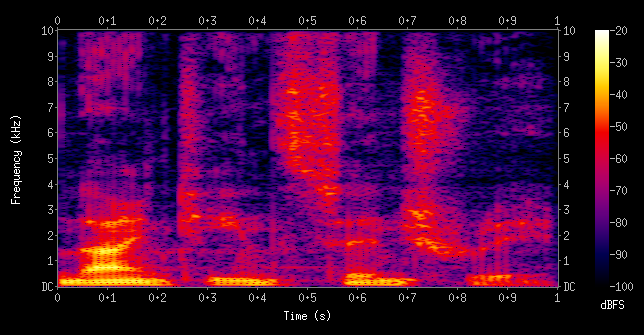
\includegraphics[width=12cm]{./Chapitre3/figures/spectrogramme.png}
  \caption{Représentation du signal en tant que spectogramme. La fréquence est modélisée en ordonnée et le temps en abscisse. L'énergie est visible grâce aux couleurs présentes: plus la couleur est chaude (rouge, orange, jaune) et plus l'énergie dégagée est importante. Image provenant de Wikipedia.}
  \label{fig:spectrogramme}
\end{figure}


Un spectrogramme est une représentation du signal audio mettant en avant l'intensité en fonction de la fréquence et du temps. %Comme on peut le voir sur la figure~\ref{fig:spectrogramme},
Il s'agit d'une représentation tridimensionnelle du signal audio. Cette transformation est possible en utilisant la transformation de Fourier qui permet de passer de l'espace temporel à l'espace fréquentiel. Les zones des énergies les plus fortes sont appellées des formants.

Cette représentation temps/fréquence peut être utilisée comme une image. Il est alors possible d'utiliser des systèmes de reconnaissance d'images afin de traiter des problématiques touchant au domaine de la parole~\cite{Stolar2017}.


\subsubsection{Coefficients Cepstraux en Fréquence Mel}
Les MFCCs, Mel-Frequency Cepstral Coefficients en anglais, sont des descripteurs spectraux utilisés très largement en traitement du signal audio, que ce soit en reconnaissance de la parole, en identification du locuteur ou en détection de concepts sémantiques par exemple. Ils sont issus d'un ensemble de traitements qui est appliqué sur le signal audio traditionnellement sur des fenêtres temporelles de 30 ms tous les 10 ms. Afin de modéliser l'évolution temporelle du signal, on utilise les dérivées premières et secondes de ces coefficients. Contrairement aux Linear Predictive Coding (LPC)~\cite{Rabiner1993},
%ou les Perceptual Linear Prediction (PLP)~\cite{Hermansky1990},
ces coefficients perceptifs sont adaptés à l'audition humaine puisqu'ils suivent l'échelle de perception de Mel. En effet, notre perception des sons n'est pas linéaire : nous percevons plus de différence entre des sons de 1000 et 2000 Hz qu'entre des sons de 7000 et 8000 Hz.

Robustes au bruit, ces coefficients permettent de représenter le spectre de façon compacte en éliminant les redondances entre les différents coefficients.

%Au total, nous avons donc une représentation en vecteurs de taille 39 pour chaque fenêtre de 10ms de signal, nous permettant de réduire considérablement le signal d'entrée, tout en gardant les informations essentielles contenues dans l'audio.

\subsubsection{Descripteurs prosodiques}
Dans le domaine du SER, il n'y a pas de consensus sur le meilleur ensemble de descripteurs à utiliser pour effectuer des tâches de reconnaissance d'émotions. C'est pour cela qu'il existe un grand nombre d'ensembles de descripteurs regroupant les différents indices acoustiques qui seront mis en relation avec les émotions. Ces indices sont soit extraits au niveau de fenêtres de courtes durées (30~ms le plus souvent), soit sur des fenêtres plus longues (plus d'une seconde) pour capturer des phénomènes para-linguistiques.

Traditionnellement, on prend un très grand nombre de descripteurs, comme par exemple l'ensemble de base extrait avec OpenSMILE~\cite{OPENSMILE}, qui compte 988 descripteurs acoustiques, puis on les filtre pour ne conserver que les plus pertinents par une sélection de descripteurs.

La sélection des descripteurs réduit la dimensionnalité de leur espace, supprime les données redondantes, non pertinentes ou bruitées. Elle apporte des effets bénéfiques directs aux systèmes : l'accélération du temps de traitement puisqu'il y a moins de données à traiter, l'amélioration de la qualité des données et donc de la performance des systèmes. De plus, elle peut permettre de rendre les résultats plus compréhensibles.
Cette sélection peut s'effectuer de plusieurs manières :
\begin{itemize}
    \item selon des méthodes de ranking, en comparant les descripteurs les uns aux autres.
    \item en utilisant des \textit{wrappers} : en utilisant le modèle de classification et en testant tous les descripteur les uns après les autres. Pour ce faire, on les enlève ou on les ajoute un à un et on sélectionne l'ensemble de descripteurs qui donne au modèle sa meilleure performance.
\end{itemize}
Néanmoins l'ordre de grandeur des corpus annotés en émotion peut vite poser problème si la dimension des descripteurs est trop importante.

Pour pallier ce problème, de plus petits ensembles de descripteurs, réalisés par des experts du domaine ont été proposés. On peut notamment citer l'ensemble INTERSPEECH 2009~\cite{Schuller2009} ainsi que \textit{The Geneva Minimalistic Acoustic Parameter Set} (GeMAPS) et sa version étendue (eGeMAPS)~\cite{Eyben2016}.

L'ensemble INTERSPEECH 2009 contient 384 descripteurs qui ont été utilisés comme référence lors du premier challenge en reconnaissance d'émotions en 2009. Il est composé de 16 descripteurs de bas niveau (Low Level Descriptors en anglais) :
\begin{itemize}
  \item \textit{zero crossing rate} : taux de passage par 0 du signal sur une fenêtre temporelle donnée.
  \item \textit{RMS energy} ou énergie moyenne quadratique : modélise la variation de l’énergie du signal à chaque fenêtre d'analyse.
  \item \textit{F0} ou fréquence fondamentale.
  \item \textit{Harmonic to noise ratio} ou rapport Harmonique-Bruit : modélise le bruit contenu dans le signal.
  \item \textit{MFCC} : les 12 premiers coefficients MFCCs sont utilisés.
\end{itemize}
Sur ces descripteurs sont calculées 12 fonctions statistiques (la moyenne, la variance, le coefficient de Pearson, de dissymétrie, le maximum, le minimum, la position relative, la plage de valeur et la régression linéaire). Soit, in fine, 16 descripteurs et leurs 16 dérivées sur lesquels on applique 12 fonctions pour un total de 384 descripteurs.

GeMAPS est composé de 18 descripteurs de bas niveau représentant des propriétés de fréquence, d’énergie, d’amplitude et des propriétés spectrales sur lesquels sont appliquées des fonctions statistiques pour un total de 62 descripteurs.
Nous reprenons la liste complète établie dans l'article de Eyben et al.~\cite{Eyben2016} dans le tableau~\ref{tab:egemaps}.

\begin{table}[h]
   \centering
   \begin{tabular}{| l |}
   \hline
       Paramètres fréquentiels \\
   \hline
       Hauteur de la voix (Pitch)  \\
       Tremblement de la voix (Jitter) \\
       Frequence des Formants 1,2,3 \\
       Bande passante (Bandwidth) des Formants 1,2,3 \\
   \hline
       Paramètres d'énergie et d'amplitude \\
   \hline
       Scintillement (Shimmer) \\
       Volume (Loudness) \\
       Ratio Harmonique-Bruit (Harmonics-to-Noise Ratio) \\
   \hline
       Paramètres spectraux \\
   \hline
       Ratio Alpha \\
       Index de Hammarberg \\
       2 pentes spectrales : 0-500Hz et 500-1500Hz \\
       Energie relative des Formants 1,2,3 \\
       Différence harmonique H1-H2 et H1-A3 \\
       MFCC 1 à 4 \\
       Flux spectral \\
   \hline
       Paramètres temporels  \\
   \hline
       Taux des pics de volume (Rate of loudness peaks) \\
       Moyenne et variance des zones parlées \\
       Moyenne et variance des zones non parlées \\
       Nombre de zones continues parlées par secondes \\
   \hline

   \end{tabular}
   \caption{Résumé des descripteurs de bas niveau (LLDs) utilisés dans l'ensemble eGeMAPS.}
   \label{tab:egemaps}
\end{table}


Comme la version courte de l’ensemble minimaliste ne contient aucun paramètre cepstral et très peu de paramètres dynamiques, on ajoute sept LLD (MFCCs, Flux spectral, Bande passante des formants 2,3) pour construire l'ensemble d'extension. En lui appliquant des fonctions statistiques, eGeMAPS contient un total de 88 descripteurs résumés dans le tableau~\ref{tab:egemaps}.
% résume toutes les caractéristiques retenues dans ces deux ensembles.

\subsubsection{Bag-of-Audio-Words (BoAW)}
Comme nous l'avons déjà indiqué, la sélection de la représentation de l'audio est un choix qui va directement influencer la qualité de la reconnaissance des émotions. C'est pour cela qu'il existe de nombreuses représentations, dont les sacs de mots-audio, ou BoAW. Inspiré des sacs de mots utilisés en NLP, il s'agit d'utiliser les LLDs sélectionnés pour former un lexique appelé \textit{codebook} de toutes les valeurs possibles, puis de les coder par un vecteur. Ce vecteur est alors utilisé en tant qu'entrée du système.

Cette solution présente comme avantage de renforcer la robustesse du système, vu que les LLDs en entrée sont en quelque sorte normalisées par ce processus. Ces features sont utilisées dans de nombreuses tâches reliées à la parole : la classification d'évènements sonores~\cite{Pancoast2012,Schmitt2016} ou la détection de plagiat~\cite{Liu2010} par exemple. Ils ont également été utilisés en reconnaissance d'émotions continues~\cite{Schmitt2016,Han2018}. %\textcolor{red}{Il manque une ref => codebook ?}.
%In this approach, feature vectors of acoustic LLDs are quantised according to a learnt codebook of audio words. Then, a histogram of the occurring ‘words’ is built.

\subsection{Descripteurs linguistiques}
Nous avons vu que lorsque l'on cherche à déterminer l'état émotionnel d'un locuteur à partir d'un enregistrement, l'approche la plus naturelle consiste à extraire des descripteurs acoustiques directement à partir du signal. On peut cependant ajouter des informations linguistiques, syntaxiques, phonémiques et sémantiques. Ces informations peuvent être extraites directement à partir d'une transcription automatique de la parole.

Les domaines du Sentiment Analysis et de l'Opinion Mining cherchent à identifier une opinion à partir d'un texte écrit. Il y a ici une différence sémantique significative entre opinion et état émotionnel, cependant les approches peuvent se rejoindre. On peut également considérer la transcription automatique comme un élément associé à la parole, et donc y retrouver des marqueurs de l'émotion. Nous détaillons dans cette partie certaines méthodes utilisées dans ces domaines pour transformer du texte (dans notre cas la transcription automatique) en descripteurs.

\subsubsection{Représentation en one-hot}
La représentation en \textit{one-hot}, comme illustrée sur la figure~\ref{fig:onehot}, correspond à associer à chaque mot un vecteur de binaires d'une taille fixe. On rassemble tous les mots-types (appelés token en anglais) utilisés dans ce que l'on nomme un vocabulaire. Puis pour chaque mot-type de ce vocabulaire, on associe un vecteur binaire unique. Cette méthode présente l'avantage d'être exhaustive et facile à mettre en œuvre, cependant la représentation est très volumineuse : le vecteur sera de la taille du vocabulaire et elle contiendra principalement des zéros.

\begin{figure}[h]
  \centering
  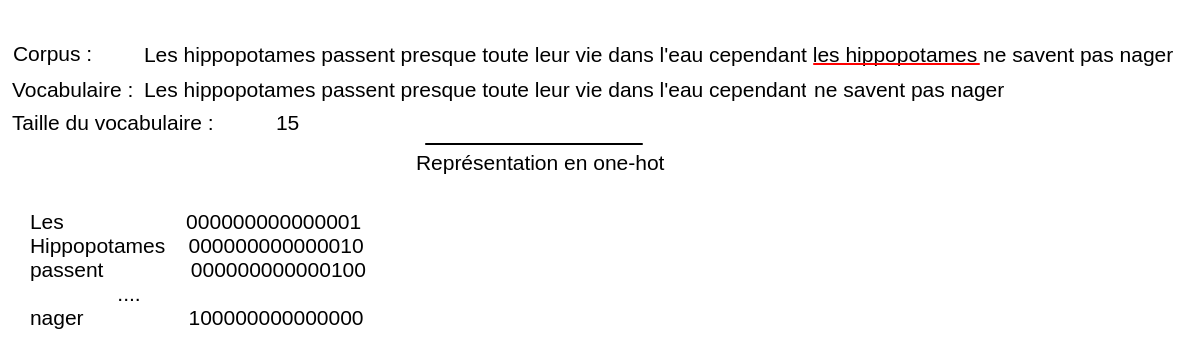
\includegraphics[width=15cm]{./Chapitre3/figures/onehot.png}
  \caption{Transformation d'un corpus en représentation one-hot.}
  \label{fig:onehot}
\end{figure}


Cette représentation permet de réaliser des opérations numériques directement sur les vecteurs \textit{one-hot}. Cependant elle ne porte aucune information sur le contexte (la position du mot-type dans la séquence), la sémantique ou sur le nombre d’occurrence de chaque mot-type.

\subsubsection{Représentation statistique}
Parmi les représentations statistiques des données textuelles, les plus courantes et les plus mises en place sont les méthodes TF (Term Frequency) et TF-IDF (Term Frequency-Inverse Document Frequency) qui prennent en compte la distribution des tokens dans les documents.
Le TF est défini comme ``the frequency of occurrence of the terms in the document or query texts''~\cite{salton_tf_idf}.
C'est-à-dire que le TF d'un mot-type $t$ présent dans un document $d$ correspond au nombre d’occurrences de $t$ dans $d$ divisé par le nombre total de tokens dans le document (Eq.~\ref{eq:tf}).
\begin{equation}
    \text{TF}(d,t) = \dfrac{\text{Nombre de } t \text{ dans } d}{\text{Nombre de tokens dans } d}
\label{eq:tf}
\end{equation}


Toujours selon Salton~\cite{salton_tf_idf}, le facteur IDF varie ``inversely with the number of documents $n$ to which a term is assigned in a collection of $N $documents. A typical idf factor may be computed as log $N/n$''.
Le facteur IDF correspond à l'inverse du rapport entre le nombre de documents où le token $t$ apparait sur le nombre total de documents $N$ (Eq.~\ref{eq:idf}).

\begin{equation}
    \text{IDF(t)} = - log\left(\dfrac{N}{\text{Nombre de documents où } t \text{ est présent} + 1} \right)
\label{eq:idf}
\end{equation}

Le TF-IDF est alors défini comme le produit des deux termes précédents comme indiqué dans l'équation~\ref{eq:tfidf}.
%Le +1 au dénominate
Pour permet d'éviter les cas où aucun document ne contiendrait le token $t$ et donc la division par zéro. Cette approche permet que les tokens qui sont soit trop fréquents, soit présents dans tous les documents, soient moins mis en avant par la représentation.

\begin{equation}
    \text{TF-IDF}(t,d) = \text{TF}(t,d) \times \text{IDF}(t)
\label{eq:tfidf}
\end{equation}

Ces méthodes statistiques ont fait leurs preuves~\cite{Martineau2009,Cambria2013,Pimpalkar2020}, même si on leur préfère maintenant des méthodes qui intègrent des aspects sémantiques notamment.

\subsubsection{Plongement de mots}
\begin{figure}[h]
  \centering
  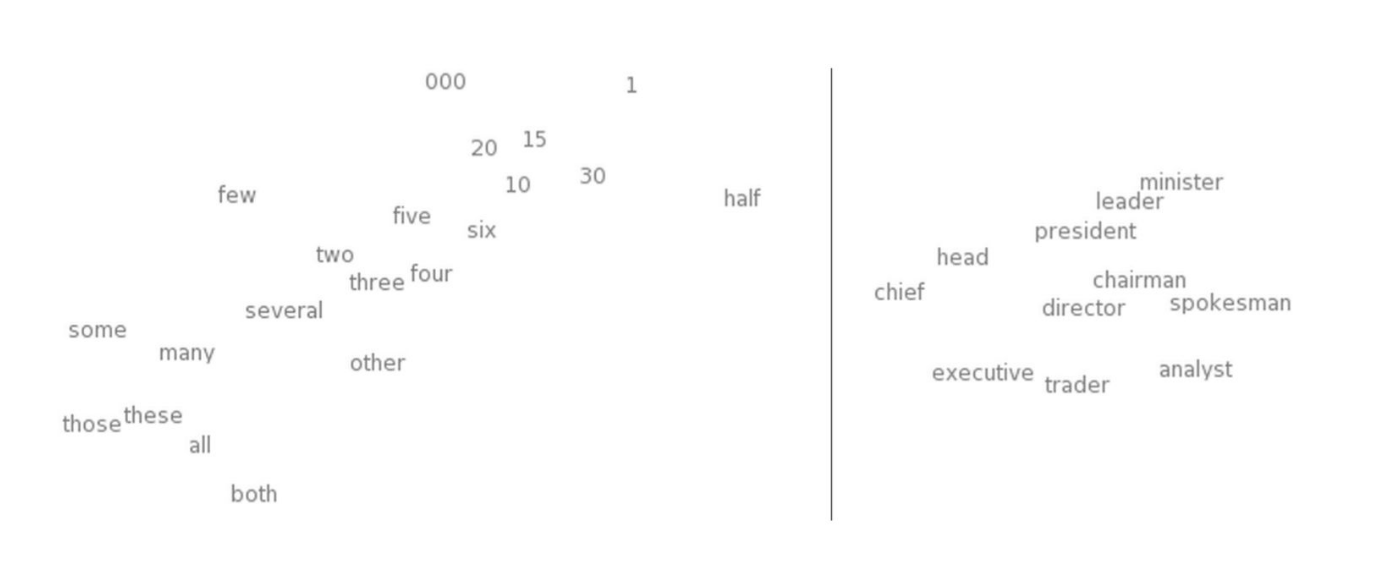
\includegraphics[width=14cm]{./Chapitre3/figures/word2vec.png}
  \caption{Représentation de plongements de mots en deux dimensions. Les mots de gauche correspondent au regroupement des termes associés au numérique. Les mots de droite correspondent aux termes associés à l'emploi. Issue des travaux de Turian et al.~\cite{Turian2010}.}
  \label{fig:word2vec}
\end{figure}


Les plongements de mots (word embeddings en anglais) ont été présentés par Bengio et al.~\cite{Bengio2003}.
A l'origine, un modèle neuronal est appris pour une tâche de reconnaissance automatique de la parole sur un grande nombre de données. Une fois le modèle entrainé, on peut prendre le réseau dans l'autre sens et supprimer les couches basses (proches de l'audio) et figer les poids afin de créer un extracteur capable de calculer des embeddings, c'est-à-dire les représentations internes du réseau de neurones, à partir d'une entrée textuelle. Ces embeddings permettent d'avoir accès à une nouvelle représentation des mots dans un espace dense et à valeurs réelles.
On projette les mots dans un espace de faible dimension, tout en isolant ensemble les mots qui ont des similarités sémantiques et syntaxiques~\cite{Ghannay2017}. Cela permet d'associer à chaque token un vecteur de valeurs réelles, de dimension bien inférieure à celle utilisée pour la représentation \textit{one-hot}. Chaque vecteur est ensuite inscrit dans un dictionnaire, et on peut alors remplacer chaque mot par le vecteur le représentant.

Leur utilisation et leur pertinence a été démontré dans de nombreuses tâches, notamment des tâches de TALN: l’étiquetage morphosyntaxique, la reconnaissance d’entités nommées, la détection de mention~\cite{Turian2010,Bansal2014} et de compréhension de la parole~\cite{Mesnil2013,Yao2014,Liu2016}.

Parmi les plongements lexicaux les plus utilisées, on trouve Word2vec~\cite{word2vec} et GloVe~\cite{Pennington2014}.
Plus précisément, les plongements de Word2Vec sont appris soit avec un algorithme de sac de mots continus (continuous bag of words, CBOW) qui prédit un mot sachant son contexte lexical, soit l'algorithme Skip-gram qui prédit les mots du contexte sachant le mot d'entrée.

Il est utile de noter que ce genre de représentation peut être visualisée dans un espace plus restreint, typiquement en deux dimensions en utilisant une réduction de dimensions (par exemple une Analyse en Composantes Principales). Ainsi les expérimentateurs peuvent observer les rapprochements sémantiques ou syntaxiques détectés par le système, comme l'illustre la figure~\ref{fig:word2vec}.

\section{Évaluation des performances}
De nombreuses métriques ont été utilisées au fur et à mesure de l'avancée du domaine pour évaluer les performances des systèmes de reconnaissance d'émotions dans la parole suivant le type de tâche : classification ou régression.

Pour les tâches de classification les métriques d'\textit{accuracy}, de précision et de rappel pondérés ou non pondérés sont les métriques les plus utilisées traditionnellement. On peut notamment se référer aux challenges INTERSPEECH en émotions de 2009 et 2011~\cite{Schuller2009,Schuller2011} qui utilisent le rappel moyen non pondéré comme métrique afin de compenser le biais de données souvent très déséquilibrées en nombre d'instances par classe.

En ce qui concerne les tâches de régression, l'erreur quadratique moyenne est une métrique efficace qui a été largement utilisée avant que des campagnes d'évaluation~\cite{AVEC2017} ne standardisent l'utilisation du Coefficient de Corrélation de Concordance (CCC) comme la mesure de référence pour l'évaluation de systèmes de reconnaissance de l'émotion continue.

\subsection{Tâche de classification}

\subsubsection{Matrice de confusion et scores associés}
La matrice de confusion est une matrice permettant de mesurer la performance d'un système de classification. Elle permet d'associer pour chaque classe de référence, les classes prédites par le système.
À chaque segment émotionnel est associée une classe qui définit l'état émotionnel de référence de la personne. Cette matrice est donc mise en place en tant qu'évaluation lorsque les émotions sont de nature discrètes. Grâce à elle, on peut retrouver les différentes erreurs du système et les quantifier. Un exemple de matrice de confusion est donné par le tableau~\ref{tab:matriceConf}. Les lignes correspondent aux références, et les colonnes aux prédictions d'un système.

\begin{table}[h]
  \centering
\begin{tabular}{|l|l|c|c|c|c||c|c|}
\cline{3-6}
\multicolumn{1}{c}{}       &         &\multicolumn{4}{c||}{\textbf{Prédiction}} \\ \cline{4-8}
\multicolumn{1}{c}{}       &             & joie        & neutre      & colère &total      &précision &rappel\\ \hline
\multirow{3}{*}{\rotatebox[origin=c]{90}{\textbf{Réf}}} &joie   & \textbf{90} & 11          & 2 &103                &0.900 &0.874\\ \cline{2-7}
                     & neutre & 4           & \textbf{80} & 10       &94        &0.889 &0.851 \\ \cline{2-8}
                     & colère & 6           & 9           & \textbf{20} &35      &0.625 &0.571 \\ \cline{2-8} \cline{2-8}
                     %& total  & 100         & 90          & 32           & & \\ \hline
\end{tabular}
\caption{Matrice de Confusion entre trois classes émotionnelles : la joie, le neutre et la colère. Les colonnes correspondent aux prédictions du système et les lignes correspondent aux références. On voit que sur 100 prédictions de la classe joie, seules 90 sont pertinentes et le système a mal prédit 13 segments qui ne devraient pas être dans la classe joie.}
\label{tab:matriceConf}
\end{table}

%\begin{figure}[h]
  \centering
  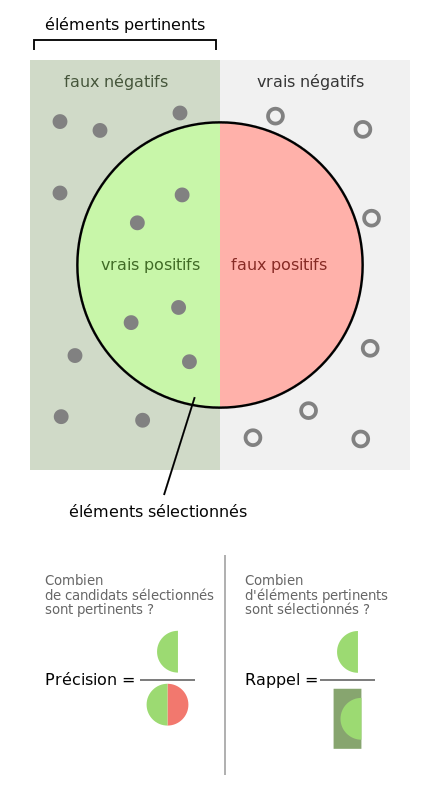
\includegraphics[width=7cm]{./Chapitre3/figures/precisionRappel.png}
  \caption{Représentation schématique de la précision et du rappel. Image provenant de Wikipedia}
  \label{fig:precisionRappel}
\end{figure}


Cette présentation permet notamment de visualiser si une classe est mieux prédite que d'autres. Il est facile de relever si le système est performant en se basant sur la diagonale, qui regroupe les vrais positifs et donc de calculer l'\textit{accuracy} définie par le nombre de segments correctement prédits sur le nombre total de segments $N$ (eq.~\ref{eq:accuracy}), tandis que les autres cases correspondent à des erreurs du système.

\begin{equation}
\text{Ac} = \dfrac{\text{Nb de prédictions vraies}}{N}
\end{equation}\label{eq:accuracy}

Cette matrice de confusion permet également de calculer le rappel et la précision de chaque classe. La précision $P_i$ de la classe $c_i$, correspond au nombre de segments de la classe $c_i$ correctement prédits parmi tous les segments prédits comme étant de classe $c_i$. (eq.~\ref{eq:precision}). Le rappel $R_i$ de la classe $c_i$ est donné par l'équation~\ref{eq:rappel} et correspond au nombre de segments correctement prédits parmi tous les segments de la classe $c_i$

\begin{equation}
  P_i = \frac{\text{nb predictions vraies}_i}{\text{nb predictions vraies}_i + \text{nb predictions fausses}_i}
  \label{eq:precision}
\end{equation}

\begin{equation}
  R_i = \frac{\text{nb predictions vraies}_i}{\text{nb segments de classe } c_i}
  \label{eq:rappel}
\end{equation}

Bien que pratique, la matrice de confusion ne permet pas de donner un score unique pour le système.


\subsubsection{Précision ou rappel pondéré et non-pondéré}

Afin d'avoir un score global de la classification des émotions, on peut moyenner les précisions et rappels par classe en pondérant ou non en fonction du nombre de segments par classe. La précision moyenne non pondérée (unweighted average precision, UAP) est obtenu en prenant simplement la moyenne des précisions par classe.
La précision moyenne pondérée (weighted average precision, WAP) est calculée en prenant la moyenne des précisions par classe suivant l'équation~\ref{eq:WA} où $N$ est le nombre de segments total et $n_i$ le nombre de segments dans la classe $c_i$. Pour éviter des possibles confusions entre les métriques de précision et de rappel, comme dans les travaux de Lee et Tashev~\cite{Lee2015} ou de Han et al.~\cite{Han2014} (où la définition de l'\textit{accuracy} par classe est ambigüe) nous indiquerons systématiquement sur quelle métrique s'applique la pondération.


\begin{equation}
  \text{WAP} = \dfrac{1}{N}\sum^n_{i=1}n_i \cdot P_i
  \label{eq:WA}
\end{equation}

La mesure de précision moyenne pondérée permet de calculer la performance d'un système de reconnaissance, mais elle ne rend pas bien compte des différences de performance entre les classes. Notamment si le corpus est déséquilibré et que le système a tendance a favoriser la classe majoritaire, on aura toujours des taux de WAP importants. Dans l'exemple du tableau~\ref{tab:matriceConf}, la classe colère n'est pas bien reconnue. Pourtant si on calcule la UAP ($\frac{0.9+0.851+0.571}{3}$) on trouve $0,774$ soit une performance élevée de $77,4\%$ de bonne prédiction. Or les prédictions de la classe colère ont une précision de $57,1\%$. L'utilisation d'une moyenne non pondérée permet de mettre en évidence ce phénomène et d'apporter une métrique plus équitable entre les différentes classes.

Nous pouvons également utiliser le rappel moyen non-pondéré, comme lors des challenges INTERSPEECH~\cite{Schuller2009,Schuller2011}. Il est calculé selon l'équation~\ref{eq:UAR} et permet de déterminer combien d'éléments pertinents ont été retrouvés.

\begin{equation}
  UAR = \dfrac{1}{n} \sum_{i=1}^n R_i
  \label{eq:UAR}
\end{equation}

\subsubsection{F-mesure}

La F-mesure, ou F-score en anglais, combine à la fois la précision et le rappel selon l'équation~\ref{eq:Fmesure}. Elle est comprise entre 0 et 1. Plus elle est grande, plus le système évalué est performant. Elle peut être calculée par classe sur les précisions $P_i$ et rappels $R_i$.

\begin{equation}
  F = 2 \left( \frac{precision.rappel}{precision+rappel} \right)
  \label{eq:Fmesure}
\end{equation}

Néanmoins toutes les reconnaissances d'émotions ne se font pas sur des émotions discrètes, il existe donc d'autres indicateurs utilisés pour mesurer la performance des systèmes.

\subsection{Tâche de régression}

\subsubsection{Erreur quadratique moyenne}
L'erreur quadratique moyenne est une métrique qui est utilisée dans l'évaluation des systèmes de reconnaissance d'émotions continues~\cite{AVEC2017}. Elle permet de calculer un score d'accord entre deux séries temporelles, ici les annotations de références et les prédictions du système. Afin que cette métrique soit de la même dimension que les valeurs de référence, on utilise principalement la racine de l'erreur quadratique moyenne, RMSE pour \textit{Root Mean Square Error}. Cette métrique se calcule selon l'équation~\ref{eq:RMSE_score} entre les valeurs prédites $x_i$  et les valeurs de références $y_i$. $n$ correspond au nombre de valeurs de la série temporelle.

\begin{equation}
    RMSE = \sqrt{\frac{1}{n}\Sigma_{i=1}^{n}{\Big(y_i - x_i\Big)^2}}
\label{eq:RMSE_score}
\end{equation}

Elle est généralement comprise entre 0 et 1 (en fonction des valeurs $x_i$ et $y_i$). Comme il s'agit d'une mesure d'erreur, les systèmes à haute performance se rapprochent de 0, ce qui indique un ajustement parfait entre les références et les prédictions. Cette métrique n'est pas exempte d'inconvénients. En effet, elle est très sensible aux valeurs extrêmes et elle est difficilement comparable à d'autre scores calculés sur des valeurs d'ordres de grandeur différents.

\subsubsection{Coefficient de Corrélation de Concordance}
Le coefficient de corrélation de concordance (CCC)~\cite{CCC} a été établi comme un standard d'évaluation lors notamment des trois précédents Audio/Visual Emotion Challenge and Workshops (AVEC)~\cite{AVEC2017,AVEC2018,AVEC2019}. Cette métrique évalue l'accord entre deux séries temporelles selon l'équation~\ref{eq:CCC_score}, où $x$ et $y$ sont les deux séries temporelles, dans notre cas la prédiction et la référence. $\mu_x$, $\mu_y$ correspondent à leur moyenne, $\sigma_x$, $\sigma_y$ à leur écart-type et $\rho$ le coefficient de corrélation entre ces deux variables aléatoires.

 \begin{equation}
    CCC = \frac{2\rho\sigma_x\sigma_y}{\sigma_x^2 + \sigma_y^2 + (\mu_x - \mu_y)^2 + \epsilon}
 \label{eq:CCC_score}
 \end{equation}

Plus le CCC s'approche de 1 et plus le système est considéré comme performant. A l'inverse, plus le score s'approche de 0 et moins il y a de corrélation entre les prédictions et les références, dénotant un système peu performant.
Cette métrique n'est pas définie dans le cas où les deux séries temporelles $x$ et $y$ sont constantes et de mêmes moyennes. On ajoute un $\epsilon$ au dénominateur pour pallier à ce problème lors de l'implémentation.

Cette métrique sera utilisée dans les travaux de cette thèse pour évaluer la performance des systèmes de prédiction continue de la satisfaction. %Afin de nuancer les différences de scores entre différentes configurations de nos systèmes, nous avons mis en place un intervalle de confiance, qui est explicité dans le chapitre~\ref{chapitre6}.

\section{Fusion de modalités}
Afin de pouvoir profiter à la fois des informations acoustiques et linguistiques, il est pertinent de fusionner ces deux modalités pour avoir un système performant et plus robuste~\cite{Wollmer2013,Alam2014,Atrey2010,Liu2018}. La fusion de modalités est assez vaste: il est possible également d'inclure des informations issues de vidéos ou de capteurs physiologiques, dont nous avons parlé au premier chapitre.

Dans le cadre de cette thèse, nous sommes principalement intéressés par les modalités acoustiques et linguistiques, puisque les autres des modalités ne peuvent pas être récupérées depuis les centres d'appels.
\\
\\
\textbf{Type de fusion}

La fusion peut s'effectuer de différentes manières.
\begin{itemize}
  \item Fusion des features~\cite{Wollmer2013,Alam2014,Atrey2010} : La fusion s'opère au niveau des features, on concatène les vecteurs représentant les différentes modalités. Cette méthode augmente le nombre de features en entrée du système et peut donner des résultats très différents en fonction de la stratégie de normalisation des données. En effet, il peut être compliqué pour le système de comprendre que les données représentent deux espaces différents. Donc il est courant de normaliser les données afin de se référer à un seul espace.
  \item Fusion des modèles~\cite{Atrey2010,Liu2018} : Plusieurs apprentissages sont faits de façon distincts pour chaque modalité jusqu'à une certaine couche dans le réseau de neurones. Les couches sont alors fusionnées, et l'apprentissage reprend. Plus la fusion arrive tôt et plus le système doit en théorie avoir un bon pouvoir de généralisation.
  \item Fusion de décision~\cite{Wollmer2013,Atrey2010} : Plusieurs apprentissages sont faits de façon distincts pour chaque modalité. On prend la prédiction de chacun des modèles et on les fusionne. S'il s'agit d'une classification, on peut fusionner par vote majoritaire par exemple. S'il s'agit d'une régression, on peut faire la moyenne des sorties. De plus, on peut facilement mettre plus d'importance sur une des modalités en faisant une moyenne pondérée des sorties.
\end{itemize}

\section{Notre référence : AVEC}

\begin{table}[]
    \centering
    \begin{tabular}{| l | l | l | c | c | c |}
        \hline
        \textbf{Models} &\textbf{Modalité} &\textbf{Features} &\multicolumn{3}{c|}{\textbf{SEWA}} \\ \cline{3-6}
        & & &activation &valence &liking \\
        \hline
        \multicolumn{6}{|l|}{AVEC 2017~\cite{AVEC2017} : Sur les conversations allemandes} \\
        \hline
        SVR      &audio &BoAW~\cite{Schmitt2016} &.344  &.351 &.081 \\
        SVR      &audio &BoTW                    &.373  &.390 &.314 \\
       \hline
       \multicolumn{6}{|l|}{Huang et al.~\cite{Huang2017} : Sur les conversations allemandes} \\
       \hline
       LSTM     &audio &eGeMAPS-88  &.506  &.455 &.193 \\
       LSTM     &audio &IS10        &.465  &.440 &.227 \\
       LSTM     &audio &Bottle-neck~\cite{Fer2015} &.533  &.466 &     \\
       LSTM     &audio &Mfcc        &.341  &.421 &     \\
       LSTM     &texte &BoTW        &.451  &.518 &.473 \\
        \hline
        \multicolumn{6}{|l|}{AVEC 2018~\cite{AVEC2018} : Sur les conversations allemandes} \\
        \hline
        biLSTM-2 &audio &eGeMAPS-88  &.124  &.112 &.001 \\
        biLSTM-2 &audio &Mfcc        &.253  &.217 &.136 \\
         \hline
       \multicolumn{6}{|l|}{Huang et al.~\cite{Huang2018} : Sur les conversations allemandes} \\
       \hline
       LSTM     &audio &eGeMAPS-88   &.497  &.438 &.281 \\
       LSTM     &audio &eGeMAPS-89   &.520  &.461 &\textbf{.335} \\
       LSTM     &audio &eGeMAPS-176  &.514  &.493 &.217 \\
       LSTM       &texte &Word2Vec-300   &\textbf{.597}  &\textbf{.600} &.454 \\
       LSTM-2     &texte &BoW            &  & &.407 \\
       LSTM-2     &texte &Word2Vec       &  & &\textbf{.480} \\
       LSTM-2     &texte &GloVe          &  & &.413 \\
        \hline
        \multicolumn{6}{|l|}{AVEC 2019~\cite{AVEC2019} : Sur les conversations allemandes et hongroises} \\
        \hline
        biLSTM-2 &audio &eGeMAPS-88  &.371 &.286 &.159 \\
        biLSTM-2 &audio &Mfcc        &.326 &.187 &.144 \\
         \hline
       \multicolumn{6}{|l|}{Schmitt et al.~\cite{Schmitt2019} : Sur les conversations allemandes} \\
       \hline
       \rowcolor{Red}
       CNN      &audio &eGeMAPS-47    &\textbf{.571}  &.517 & \\
       \rowcolor{Red}
       biLSTM-4 &audio &eGeMAPS-47    &.568  &\textbf{.561} & \\
       \hline
    \end{tabular}
    \caption{Compilation des scores de CCC sur l'ensemble de développement de SEWA sur les 3 dimensions : activation, valence et \textit{liking}. L'acronyme BoAW signifie \textit{Bag-of-audio-words}, BoTW signifie \textit{Bag-of-text-words}, SVR signifie Support Vector Regression~\cite{Smola2004}, proche des SVM mais applicable à des problèmes de régression et donc à une annotation continue. Les différents nombres associés aux features de type eGeMAPS dénotent de différentes configurations utilisées autour de ces sets : soit avec une sélection reduite des LLDs (47), soit avec l'ajout d'information sur le locuteur courant (89 et 176).}
    \label{tab:avec}
\end{table}

Si nous nous replaçons dans le contexte de la thèse, nous cherchons à construire et donc à évaluer un système de reconnaissance des émotions continues depuis la parole. Dans ce cadre, nous avons recherché dans la littérature, des systèmes et des expérimentations qui soient comparables à nos recherches. Nous avons choisi de nous référer aux campagnes AVEC, \textit{Audio/Visual Emotion Challenge and Workshop}.

Ce challenge, qui en était à sa huitième itération en 2018, vise à comparer les méthodes de traitement multimédia et d'apprentissage automatique pour l'analyse automatique de la santé et des émotions dans les modalités audio et visuelles. Ces campagnes sont divisées en différents objectifs qui gravitent autour des émotions: de la détection de dépression, de bipolarité, d'état d'esprit ou d'émotions issues de différentes cultures par exemple. Comme ces campagnes s'appuient sur des corpus multimodaux comme RECOLA~\cite{Ringeval2013} et SEWA~\cite{SEWA} notamment, les émotions peuvent être détectées à partir de différentes modalités, notamment depuis la parole et les expressions faciales.

Afin de pouvoir nous comparer à l'état de l'art, nous avons décidé de comparer nos résultats à ceux obtenus sur le corpus SEWA, dont nous avons parlé dans ce chapitre.
Ce corpus considère trois dimensions émotionnelles : la valence, l'activation et le \textit{liking} qui correspond à l'appréciation par les participants des clips visionnés en amont. Il est utilisé notamment dans les campagnes AVEC depuis 2017~\cite{AVEC2017,AVEC2018,AVEC2019} et sert actuellement de baseline dans la communauté. Nous nous intéressons donc à la tâche de régression audio uniquement.

Nous résumons dans le tableau~\ref{tab:avec}, différents résultats obtenus qui utilisent la partie Allemande et Hongroise du corpus, soit celle à laquelle nous avons accès. Comme nous pouvons le voir, de nombreux ensembles de features et types d'algorithme ont été utilisés pour la reconnaissance des émotions depuis la parole pour le corpus SEWA.
Pour ce qui est de la modalité acoustique, nous pouvons voir que les systèmes les plus performants ont des scores de 0.571 pour l'activation, 0.561 pour la valence et 0.335 pour le liking. Nous voyons que la plupart des participants ont utilisé des systèmes CNN ou LSTM (détaillés dans le chapitre~\ref{chapitre5}) pour résoudre la régression. En regardant les deux études de Huang et al.~\cite{Huang2017,Huang2018}, nous pouvons remarquer que le choix de l'ensemble de descripteurs influence fortement sur les scores des systèmes de regression. On remarque également une prédominance de l'utilisation des eGeMAPS, qui donne les meilleurs scores.

Pour ce qui est de la modalité linguistique, on peut notamment remarquer que l'on retrouve principalement l'utilisation de plongements de mots (word2vec et GloVe) et le même type d'architecture que pour la modalité acoustique, avec une variation du réseau LSTM, qui possède deux couches pour les expérimentations sur le liking.

Si on compare les résultats à ceux trouvés par la modalité acoustique, les scores maximum sont assez similaires : 0.597 contre 0.571 pour l'activation, 0.600 contre 0.561 pour la valence. On observe également une nette amélioration pour le liking : 0.480 au lieu de 0.335. En général, on trouve des scores un peu plus élevés en utilisant la modalité linguistique~\cite{Gunes2013}. Cela peut être dû au fait que les descripteurs utilisés sont plus adaptés ou que les architectures neuronales sont plus adaptées à ce type de données.

Dans le cadre de cette thèse, nous cherchons à mettre en place des solutions neuronales profondes. Nous avons donc fait le choix de nous comparer aux résultats obtenus par Schmitt et al.~\cite{Schmitt2019} correspondant aux lignes rouges du tableau.
%\begin{table}[]
    \centering
    \begin{tabular}{| l | l | c | c | c |}
        \hline
        \textbf{Models} &\textbf{Features} &\multicolumn{3}{c|}{\textbf{SEWA}} \\ \cline{3-5}
        & &activation &valence &liking \\
        \hline
        \multicolumn{5}{|l|}{AVEC 2017~\cite{AVEC2017} : Sur les conversations allemandes} \\
        \hline
        SVR      &BoTW       &.373  &.390 &.314 \\
       \hline
       \multicolumn{5}{|l|}{Huang et al.~\cite{Huang2017} : Sur les conversations allemandes} \\
       \hline
       LSTM     &BoTW        &.451  &.518 &.473 \\
        \hline
       \multicolumn{5}{|l|}{Huang et al.~\cite{Huang2018} : Sur les conversations allemandes} \\
       \hline
       LSTM       &Word2Vec-300   &\textbf{.597}  &\textbf{.600} &.454 \\
       LSTM-2     &BoW            &  & &.407 \\
       LSTM-2     &Word2Vec       &  & &\textbf{.480} \\
       LSTM-2     &GloVe          &  & &.413 \\
       \hline
    \end{tabular}
    \caption{Compilation des scores de CCC sur l'ensemble de développement de SEWA sur les 3 dimensions : activation, valence et \textit{liking}. L'accronyme BoTW signifie \textit{Bag-of-text-words}, SVR signifie Support Vector Regression~\cite{Smola2004}, proche des SVM mais applicable à des problèmes de régression et donc à une annotation continue.}
    \label{tab:avectexte}
\end{table}


% \section{Sentiment Analysis et Opinion Mining}
% Utiliser le texte pour déterminer l'état émotionnel est une voie de plus en plus empruntée grâce, notamment, à la performance des systèmes de reconnaissance de la parole actuels.
% Des domaines tels que l'Analyse de Sentiments et la Détection d'Opinion, utilise des données textuelles de type livres, témoignages ou plus récemment des tweets et  des contenus en ligne afin d'extraire des informations. On peut également considérer la transcription automatique comme un élément associé à la parole, et donc y retrouver des marqueurs de l'émotion.
%
% Dans ces domaines, on cherche alors l'émotion dans l'aspect sémantique de la phrase, dans les diffluences ou les répétitions.
%
% Le terme \textit{Détection d'Opinion} (traduction de Opinion Mining) a été popularisé par les travaux de Kushal Dave~\cite{Dave2003}, définissant le domaine comme traitant un ensemble de données pour en retirer ses qualités et ses caractéristiques afin de statuer sur l'avis du sujet~\cite{Pang2008}. Le domaine \textit{Analyse de Sentiments} (traduction de Affect Analysis) a pris de l'ampleur depuis les travaux de Sanjiv Das, Mike Chen et Richard Tong au début du XXIe siècle~\cite{Das2007,Tong2001}. Il diffère de l'Opinion Mining : la majorité de ces travaux se concentrent sur la classification des avis ou de phrases en polarité (positif ou négatif). Mais ces domaines de recherche restent très fortement liés et constituent la plus grande partie de recherche d'indices émotionnelles à base de données textuelles.
%
% Des outils tel que des dictionnaires de polarité, FAN~\cite{Monnier2014} par exemple, permettent de colorer émotionnellement des mots ou des phrases, ou encore des analyseurs de syntaxe tel que Macaon~\cite{Nasr2011} permettent d'étudier la structure d'un énoncé pour faire ressortir sa forme morphosyntaxique. Ces outils sont utilisés dans la reconnaissance d'émotions que ce soit à l'échelle d'un segment de parole, d'une phrase ou d'un document.
%
% \subsection{Corpus existant}
% De nombreux corpus de texte existent, mais peu sont annotés en émotion. Si nous nous référons aux campagnes AVEC, la transcription automatique de la parole est utilisée en tant que donnée textuelle. Cette transcription est ensuite alignée aux annotations, permettant d'obtenir ainsi des données annotées.
%
% Il est également possible de constituer son propre corpus en confrontant un texte à des lexiques d'émotions comme par exemple le lexique NRC~\cite{Mohammad2013} disponible dans 105 langues, SentiWordNet~\cite{Sebastiani2006} ou encore le lexique FAN~\cite{Monnier2014}.
% Le lexique NRC contient 14 182 mots et sont associés à 10 catégories différentes (anticipation, colère, tristesse, joie, peur, confiance, dégoût, surprise, positive, négative). Chaque mot peut être associé à plusieurs catégories ou à aucune.
% Le dictionnaire French Affective Norms (FAN) propose quant à lui, un score de valence (entre 0 et 10) pour plus de 1000 mots, annotés par plus de 400 participants.
%
% Il est également possible de se tourner vers des corpus déjà construits, comme ceux utilisés lors des campagnes SemEval. Par exemple des titres d'article provenant de journaux~\cite{Strapparava2010} ou encore un corpus constitué de livres pour enfants~\cite{Etienne2020}. Les données de SemEval sont annotés en catégories discrètes (colère, dégoût, peur, joie, tristesse, surprise et valence) par une échelle allant de 0 à 100 pour chaque émotion. 0 signifiant l'absence de l'émotion dans le titre et 100 la charge émotionnelle maximale. La valence varie entre -100 (négative) et 100 (positive) avec 0 (neutre) au milieu. Le corpus de livres pour enfants est annoté en 10 catégories discrètes (colère, dégoût, joie, peur, surprise, tristesse,culpabilité, embarras, fierté et jalousie). Cette annotation est enrichie en plusieurs concepts, notamment le mode d'expression de l'émotion : désignée, comportementale, montrée, étayée.
%
% De nombreux autres corpus existent afin de traiter un maximum de tâches en lien avec les émotions. Mais ces corpus sont difficilement utilisables en l'état, il est important de les transformer afin de les rendre compréhensibles par les systèmes d'apprentissage.

% \subsection{Les scores de systèmes à l'état de l'art tirés d'AVEC}
%
% \begin{table}[]
    \centering
    \begin{tabular}{| l | l | c | c | c |}
        \hline

       \hline
    \end{tabular}
    \caption{J'ai pas retrouvé de scores pour la fusion acoustiques et linguistiques. On a toujours de la vidéo dedans.}
    \label{tab:avecmulti}
\end{table}

%
% Une fois encore, nous nous intéressons aux scores présentés lors du challenge AVEC. La multi-modalité étant un aspect prédominant dans cette campagne, les données comportent également des vidéos qui peuvent être utilisés par les participants. Dans le tableau~\ref{tab:avecmulti}, nous ne rapportons que les scores des modalités acoustiques et linguistiques.

\section{Conclusion}
Dans ce chapitre, nous avons résumé les principaux composants de la reconnaissance des émotions depuis la parole, sans oublier la reconnaissance depuis le texte. A partir de ces connaissances, nous avons pu établir un référentiel sur la tâche que nous cherchons à accomplir. En effet, nous avons fait le choix de nous comparer au corpus SEWA et aux différents systèmes et features utilisés avec celui-ci. De plus, nous avons introduit le principe de fusion des modalités, qui apparaîtra dans les contributions de cette thèse.

Dans la prochaine partie, nous allons nous concentrer sur les contributions de cette thèse : de la construction d'un corpus répondant à nos besoins, à la mise en place de systèmes de reconnaissance des émotions performants et l'analyse des résultats obtenus.
